\section{The Bottleneck: Retrieval Precision, then Reasoning}
\label{sec:bottleneck}

To locate the lost accuracy we exploit LoCoMo's per-question \emph{gold
evidence} turn ids, which most work ignores. We compare, per question
($n{=}200$, LLM-judged):
\begin{itemize}
  \item \textbf{retrieved}: our top-$k$ pipeline ($k{=}12$);
  \item \textbf{oracle}: only the gold evidence turns (with session dates) in
  context---a perfect-retrieval ceiling;
  \item \textbf{full\_conv}: the entire multi-session conversation in context
  (no retrieval), with \texttt{num\_ctx}$=32768$ so nothing is truncated.
\end{itemize}

\paragraph{Retrieval precision leaves large headroom.}
Overall accuracy is $0.40$ (retrieved) vs.\ $0.61$ (oracle)---about $21$ points
lost to imperfect retrieval---and on multi-hop the gap is $0.41\!\to\!0.72$
(Table~\ref{tab:oracle}). This is real, measured headroom for a precision
retriever, consistent with recent conversational-memory retrieval
work~\cite{li2026evimem,ji2026mragent}.

\paragraph{Precision beats recall: more context distracts.}
Supplying the whole conversation is \emph{worse} than precise evidence on
multi-hop ($0.628$ vs.\ $0.721$), echoing distraction
effects~\cite{liu2023lost,cuconasu2024power}. The lever is retrieving the exact
evidence, not retrieving more.

\paragraph{Reasoning is a hard floor retrieval cannot cross.}
On temporal questions, even the oracle scores only $0.156$: the gold evidence
and session dates are present, but the model cannot perform the required date
arithmetic (e.g.\ ``yesterday'' relative to the session date). No retriever can
fix this---it is a reasoning/grounding limit, and it caps how much precision
retrieval alone can deliver.

\begin{figure}[t]
\centering
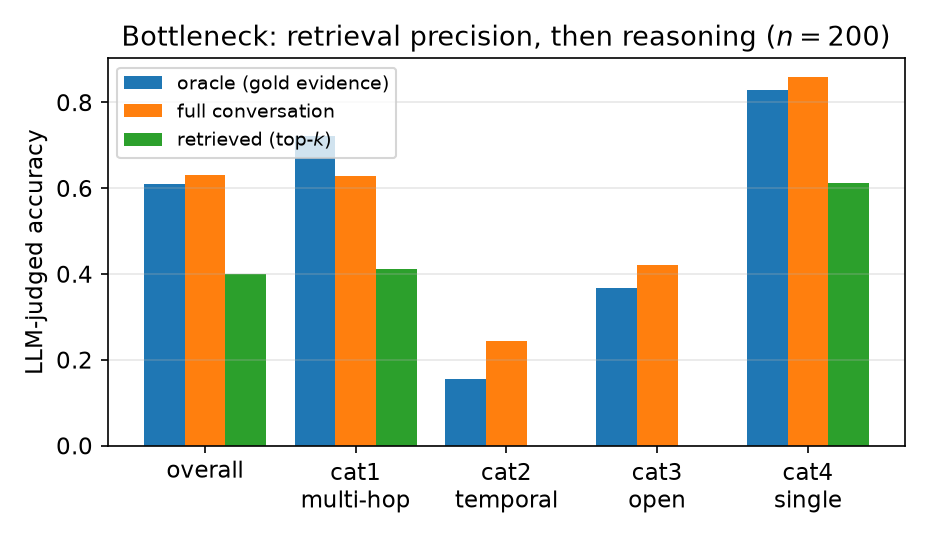
\includegraphics[width=\linewidth]{figures/fig_oracle.png}
\caption{Bottleneck decomposition ($n{=}200$). Oracle (gold evidence) far
exceeds retrieval, but temporal stays near-floor even with perfect evidence,
and full-context underperforms the oracle on multi-hop.}
\label{fig:oracle}
\end{figure}

\begin{table}[t]
\centering
\small
\begin{tabular}{lccccc}
\toprule
arm & overall & cat1 & cat2 & cat3 & cat4 \\
 & & (multi) & (temp) & (open) & (single) \\
\midrule
retrieved ($k{=}12$) & 0.400 & 0.411 & -- & -- & 0.613 \\
oracle & 0.610 & \textbf{0.721} & \textbf{0.156} & 0.368 & 0.828 \\
full\_conv & 0.630 & 0.628 & 0.244 & 0.421 & 0.860 \\
\bottomrule
\end{tabular}
\caption{Bottleneck decomposition ($n{=}200$, LLM-judged). Retrieval precision
leaves $\sim\!21$ points on the table; full-context \emph{distracts} on
multi-hop; temporal reasoning is near-floor \emph{even with gold evidence}.}
\label{tab:oracle}
\end{table}

\paragraph{Takeaway.} Effort ordering for small-model conversational memory:
deduplication (no effect) $<$ precision retrieval (bounded but real) $<$
reasoning/grounding (the ceiling). The temporal floor in particular is a
retrieval-invariant limit.
